\chapter{Implementación}
     En este capítulo se explican los detalles de la implementación de las partes \textit{frontend} y \textit{backend} de nuestro proyecto, tanto de la generación del proyecto inicial como de la infraestructura del mismo.
    
    
    \section{Frontend}
    En esta sección se va a hablar del proyecto Angular el cual compone la parte \textit{frontend} de nuestra aplicación. Este \textit{framework} nos ofrece un desarrollo más rápido con respecto a otros \textit{frameworks}, ya que se estructura en diferentes componentes web y genera una página web dinámicamente.
    \subsection{Generación Proyecto Angular}
    Para la generación de un proyecto base en Angular se utilizó \textit{Angular Cli}, un herramienta de línea de comandos que facilita la creación y gestión de proyectos Angular y de sus diferentes componentes.
    \newline
    
    \textit{Angular Cli}, al tratarse de  una herramienta NodeJS, requiere tenerlo instalado en nuestro sistema operativo. Para ello la primera tarea a realizar es instalar NodeJS a través de su página oficial\cite{nodejs}, escogiendo la versión que soporte nuestro sistema operativo.
 
    A continuación, a través del terminal que nos proporciona la herramienta de desarrollo \textit{Visual Studio Code}, ejecutamos el comando \texttt{npm install -g @angular/cli@latest}, el cual nos instala \textit{Angular Cli} en la última versión disponible.
    
    \begin{figure}[h]
    \centering
     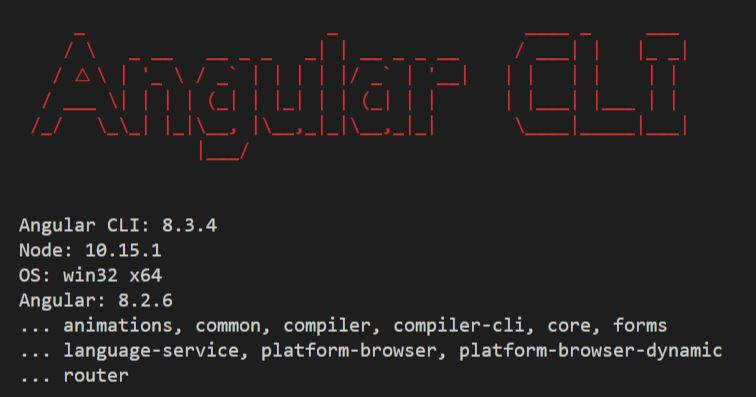
\includegraphics[width=0.65\textwidth]{images/angularversion}
    \caption{Versión Angular Cli}
    \end{figure}
    
    \FloatBarrier
    
    Una vez instalada la herramienta de comandos \textit{Angular Cli}, procedemos a crear nuestro proyecto base Angular ejecutando el comando \texttt{ng new estudio-medico-tfg2019}, generando un proyecto completo Angular junto con toda su estructura de carpetas.
    
    
    
    \subsection{Arquitectura de la aplicación Angular}
    
    Angular es una herramienta que se sustenta en la idea de modular del código en componentes. Estos componentes son fragmentos de código independientes que la pagina web carga o descarga según las acciones del usuario. 
    
    \begin{figure}[h]
    \centering
     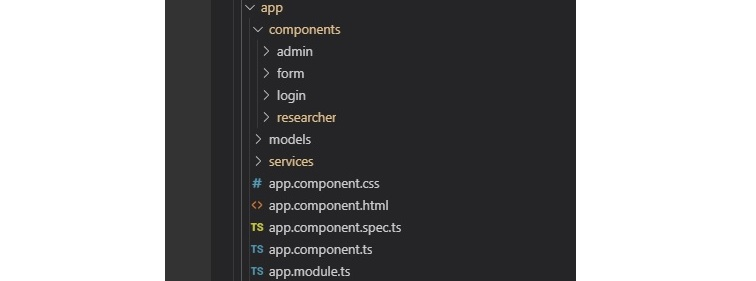
\includegraphics[width=1\textwidth]{images/componentesAngular.jpg}
    \caption{Estructura de componentes en Angular.}
    \end{figure}
    
     \FloatBarrier
    
    En el caso de nuestro proyecto se emplearon cuatro grandes componentes (admin, form, login y researcher) así como algunos mas pequeños que se desglosarán más adelante. El componente app que los engloba es creado por Angular automáticamente y sirve como base para montar y desmontar el resto de componentes.
    
    \subsubsection{\underline{login}}

    El primer componente que se creó en la aplicación y sobre el que se desarrolló el diseño general que se seguiría en el resto de la misma. Como todos los componentes de esta aplicación se compone de un archivo HTML con la estructura del elemento, un archivo CSS con el diseño del mismo y finalmente un archivo de TypeScript con los comportamientos posibles del componente.\newline
    
    \begin{figure}[h]
    \centering
     
\includegraphics[width=1\textwidth]{images/loginComponent.jpg}
    \caption{Estructura del componentes de login.}
    \end{figure}
    \FloatBarrier
    
    En cuanto a la estructura el elemento se compone solamente de la cabecera, un formulario para introducir usuario y contraseña y un modal para mensajes de error. Aprovecharemos que este es uno de los formularios más sencillos de la aplicación para explicarlo un poco más en detalle, ya que estos son una parte fundamental de la misma.
    
    \begin{figure}[h]
    \centering
     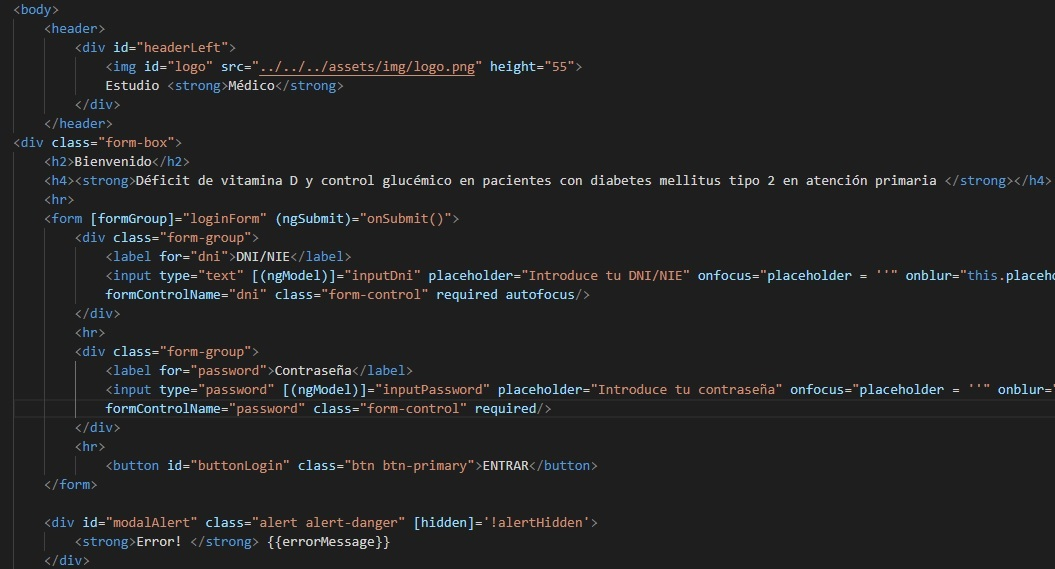
\includegraphics[width=1\textwidth]{images/loginHTML.jpg}
    \caption{Código HTML del login.}
    \end{figure}
    \FloatBarrier
    
    Los formularios constan de un formGroup con nombre propio (loginForm en este caso) que engloba uno o varios elementos de control con nombre propio (formControlName, en este caso dni y password) como campos de entrada de datos para el formulario y finalmente un botón para disparar la validación del formulario, cuyo resultado se representa como mensaje de error en el modal que hay justo a continuación o con la resolución del mismo, que en este caso permitiría acceder a la aplicación con el perfil introducido. Este proceso de validación y respuesta se produce en el archivo de TypeScript.
 
    \begin{figure}[h]
    \centering
     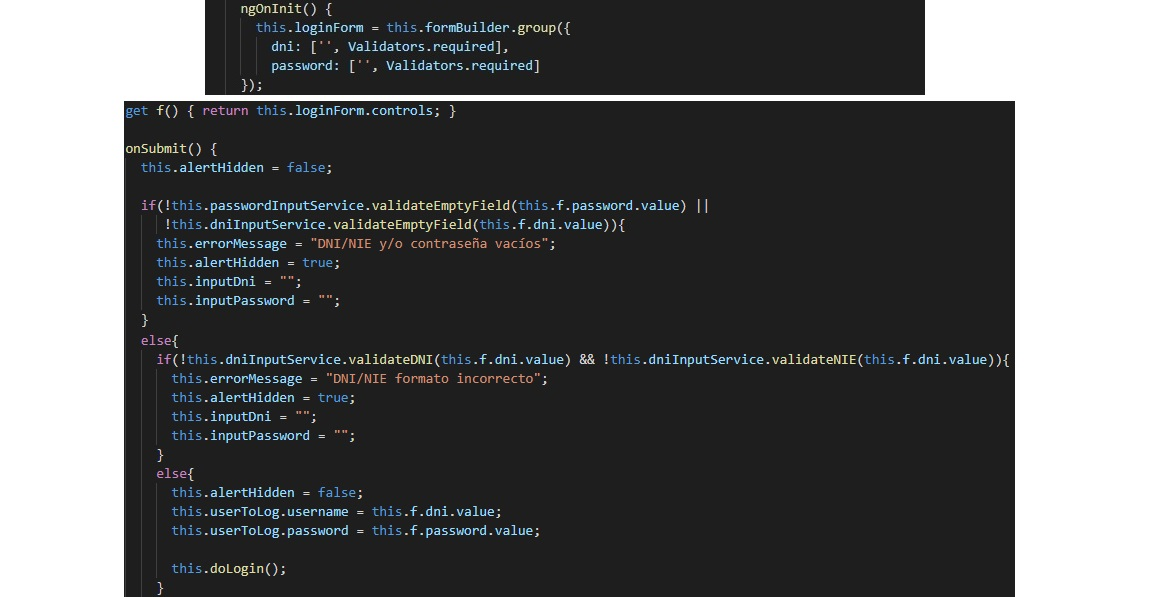
\includegraphics[width=1\textwidth]{images/loginTS.jpg}
    \caption{Código TypeScript del login.}
    \end{figure}
    \FloatBarrier
    
    En la figura anterior se observan dos bloques, uno es el del método ngOnInit, que es lanzado por el componente justo al montar la página y enlaza los campos del formGroup explicado anteriormente con las variables que se utilizan en este archivo mediante sus nombres (dni y password). El segundo bloque recoge el método onSubmit que se lanza al presionar el botón del formulario y como se puede apreciar primero realiza las validaciones, las cuales en caso de ser erróneas rellenan el modal con un mensaje de error, y finalmente llama al método doLogin que conecta al usuario a la aplicación si todas han sido correctas. Sin embargo estas validaciones son llamadas desde dos elementos externos a este documento, el dniInputService y el passwordInputService. Estos servicios son una colección de métodos que no se encuentran dentro de ningún componente y  sirven tanto para ser utilizados de forma recurrente por cualquiera de estos como para conectar la aplicación Front al \textit{backend}.
    
    \begin{figure}[h]
    \centering
     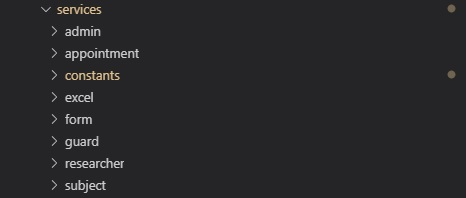
\includegraphics[width=1\textwidth]{images/services.jpg}
    \caption{Servicios disponibles en la aplicación.}
    \end{figure}
    \FloatBarrier
    
    Al igual que los componentes, los servicios están englobados en cuatro grandes grupos: admin y reseracher, los dos perfiles existentes en la aplicación y subject y form, los dos elementos principales a manejar en la misma. El resto de grupos de servicios corresponden a métodos puntuales que no encajaban en ninguno de estos grupos, de los cuales hablaremos según vayan apareciendo. En el caso del login sus servicios están incluidos en el grupo de researcher, ya que fue el primer perfil para el que se diseñó el mismo.
    
     \begin{figure}[h]
    \centering
     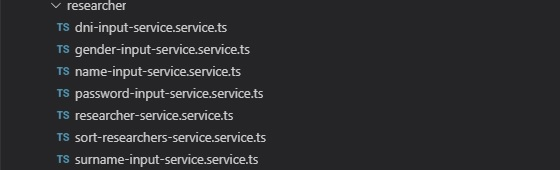
\includegraphics[width=1\textwidth]{images/researcherService.jpg}
    \caption{Servicios asociados al perfil de investigador.}
    \end{figure}
    \FloatBarrier
    
    Estos servicios engloban las validaciones de campos (los servicios con el sobrenombre input) tanto para hacer login en la aplicación como para registrar investigadores. El servicio researcher-service comprende todos los métodos de acceso al \textit{backend} referentes a este perfil.\newpage
    
    \subsubsection{\underline{form}}
    
    El componente de formulario se compone de dos partes: un componente appointment que engloba el test a realizar en los pacientes durante las citas y el appointment-view que es una visualización no editable del mismo una vez completado.
    
    \begin{figure}[h]
    \centering
    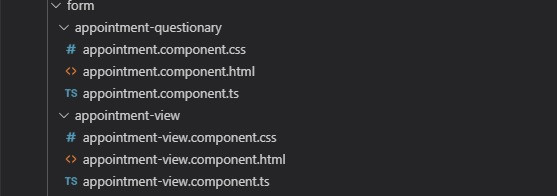
\includegraphics[width=1\textwidth]{images/formComponent.jpg}
    \caption{Componentes del test para las citas y su visualización una vez completados.}
    \end{figure}
    \FloatBarrier
    
    El primer componente corresponde al formulario de la figura, el cual tiene una estructura similar a la explicada para el de login solo que con una longitud de 600 líneas. Así mismo, tiene un componente de TypeScript en el que se manejan las validaciones, mensajes de error y el guardado del contenido en la base de datos. Se sirve de los servicios del form-service para realizar las validaciones de todos sus campos y de varios métodos del researcher-service para realizar los accesos a la base de datos a través del \textit{backend}.
    
    \begin{figure}[h]
    \centering
    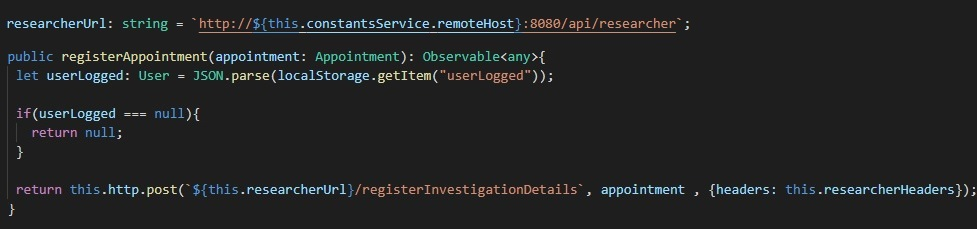
\includegraphics[width=1\textwidth]{images/registerAppointment.jpg}
    \caption{Método para el guardado del test referente a una cita completada.}
    \end{figure}
    \FloatBarrier
    
    En la figura anterior se puede observar el método encargado de guardar la información del test en el sistema. Utiliza una url para saber donde encontrar el \textit{backend} que le está ofreciendo los métodos, en la cual se utiliza una variable externa exportada desde constantService. Esta variable simplemente sirve como manera rápida de cambiar entre la url de acceso local, con la que los desarrolladores pueden trabajar en sus bases de datos privadas, y la url que conecta con el servidor operativo en Hostinger. Mediante la terminación de esta url, que se añade dentro de cada método, el \textit{backend} es capaz de distinguir a qué controlador y qué método esté haciendo la llamada el \textit{frontend}, el cual además le pasa los datos (en este caso el test relleno) como un parámetro junto a la llamada.\newline
    
    El segundo componente corresponde a la figura 4.20 y es solo la visualización de los datos de un test ya realizado, obtenidos en una sola llamada al cargar el componente y no comprende ningún otro comportamiento.\newpage
    
    \subsubsection{\underline{admin}}
    
    El siguiente componente incluye todas las vistas del perfil de administrador. Comprende cuatro componentes, uno para cada elemento de la aplicación (investigadores, pacientes y test) y uno para la edición de perfiles de investigadores.
    
    \begin{figure}[h]
    \centering
    
\includegraphics[width=1\textwidth]{images/adminComponents.jpg}
    \caption{Componentes relacionados con el perfil de administrador.}
    \end{figure}
    \FloatBarrier
    
    El primer componente corresponde a la vista con el listado de test realizados en la aplicación por todos los investigadores y a la figura 4.24, que es la modificación de una de estas. Para el componente del listado se trae de la base de datos todos los test realizados con el investigador que los realizó y se rellena una tabla dinámicamente con dicha información.
    
    \begin{figure}[h]
    \centering
    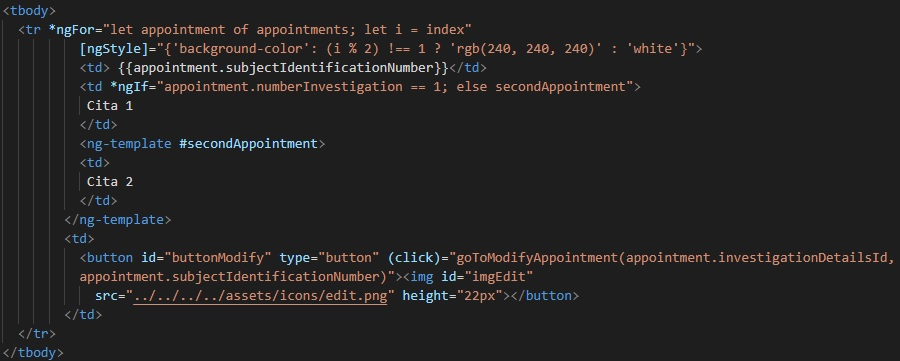
\includegraphics[width=1\textwidth]{images/appointmentTable.jpg}
    \caption{Bucle de generación para la tabla de test realizados.}
    \end{figure}
    \FloatBarrier
    
    La tabla emplea una variable en el archivo de TypeScript asociado en la que se han guardado los test llamada appointments (al principio del bucle for) y para cada iteración escribe el número de identificación del paciente, si es el test es de su cita 1 o 2 y un botón de editar que permite abrir la vista al segundo componente.\newline
    
    El siguiente componente de administrador es edit-researcher-admin, que es una sencilla vista con un formulario que permite editar nombre, apellidos y la contraseña de un investigador que se puede ver en la figura 4.16. A este componente se accede mediante una tabla, muy similar a la utilizada para los test, que se encuentra en el componente de researcher-admin. Este es a su vez la vista principal del administrador nada más identificarse en la aplicación y contiene dicha tabla de investigadores y un formulario que se puede observar en la figura 4.11 que permite el registro de investigadores. El último componente, referente a los pacientes, incluye una tabla en la  línea de las anteriores y unos filtros para la misma como se puede ver en la figura 4.18.\newpage
    
    \subsubsection{\underline{researcher}}
    
    El último grupo de componentes son los referentes al perfil de investigador. En este grupo se añadiría el componente de estadísticas comentado en capítulos anteriores.
    
    \begin{figure}[h]
    \centering
    
\includegraphics[width=1\textwidth]{images/researcherComponent.jpg}
    \caption{Componentes relacionados con el perfil de investigador.}
    \end{figure}
    \FloatBarrier
    
    Como se observa en la figura anterior existen dos componentes para este perfil. El primero implementa la vista principal del investigador, donde ve una tabla con los pacientes que tiene asociados y un pequeño campo para introducir nuevos pacientes mediante su código de identificación como se puede ver en la figura 4.8. Incluye también un modal para mensajes de error y un formulario de inclusión. Este formulario mediante CSS aparece sobre el resto del contenido al añadir un paciente para solicitar que marques si se cumplen todos los criterios de admisión (mayor de 18 años, al menos una visita previa en el centro, etc). Aprovecharemos este componente para explicar como se manejan los errores y las llamadas de observables.
    
    \begin{figure}[h]
    \centering
    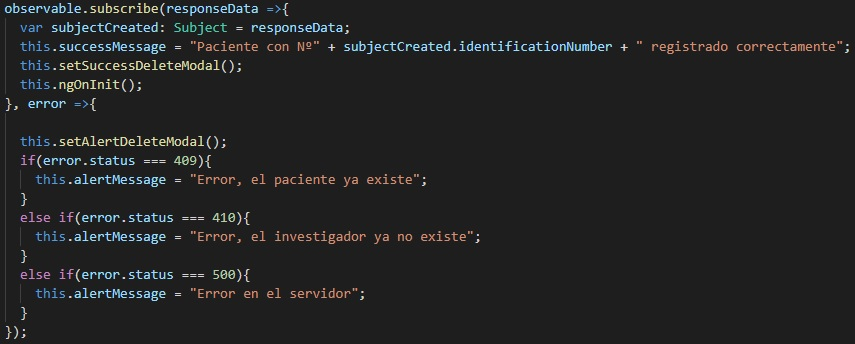
\includegraphics[width=1\textwidth]{images/observableAndErrors.jpg}
    \caption{Llamada a un servicio mediante un observable y manejo de errores.}
    \end{figure}
    \FloatBarrier
    
    En la figura vemos como un observable utiliza un método subscribe que dentro incluye el código del que hablaremos. Este observable es básicamente una llamada asíncrona a un método, en este caso registrar paciente, a la cual nos suscribimos para manejar su resultado cuando se obtenga. Dentro del método vemos un primer bloque de código para responseData, el cual es llamado en caso de devolver el método a parte de su contenido un código HTTP 200, que significa que todo ha ido sin problemas. En caso de devolver otro código se accede al segundo bloque en el que se activa el modal con el mensaje de error y se muestra una explicación del mismo más ilustrativa que solo un número. Estos códigos de error han sido decididos por los desarrolladores siguiendo la filosofía original de HTTP y por ese motivo se conoce exactamente cuales se pueden dar y su significado.\newpage
    
    \subsection{Inicialización del proyecto}
    
        \subsubsection{\underline{Local}}
        
        Para la inicialización del proyecto en local es necesario tener algún entorno de desarrollo compatible, como Visual Studio Code el cual hemos utilizado nosotros, y tener instalada la interfaz de línea de comandos de Angular (Angular CLI). Una vez instalada solo necesitamos abrir el proyecto en nuestro entorno, abrir un terminal y ejecutar \texttt{ng serve}. En ocasiones el instalador de paquetes npm tiene problemas para reconocer el comando (nos ha ocurrido en algunos equipos) y sera necesario escribir una sentencia algo más completa: \texttt{npm run ng serve}.
        \subsubsection{\underline{Remoto}}
        En el caso de querer acceder a la aplicación en remoto no se requiere de ningún requisito previo más que utilizar un navegador. La página desde la que se accede a la aplicación es http://tfg-estudio-medico.com/
    
    
    \section{Backend}
    
     En esta sección se va a hablar del proyecto Java Spring Boot el cual compone la parte \textit{backend} de nuestra aplicación. La aplicación es una API-REST, la cual será consumida por el \textit{frontend} mediante llamadas en protocolo HTTP. 
     
     
    \subsection{Generación Proyecto Java Spring Boot}
    Para la generación del proyecto inicial se utilizó Spring Initializr\cite{springinitializr}, a través de su página web. Escogimos gestionar las dependencias del proyecto con Maven dado el alto grado de familiaridad que poseemos con esta tecnología. A continuación se escogió el lenguaje Java para implementar la aplicación debido a sus características intrínsecas(polimorfismo y herencia). Para finalizar se añadieron los paquetes de Web y JPA, necesarios para gestionar las conexiones externas y para la capa de persistencia.
    
    \begin{figure}[h]
    \centering
     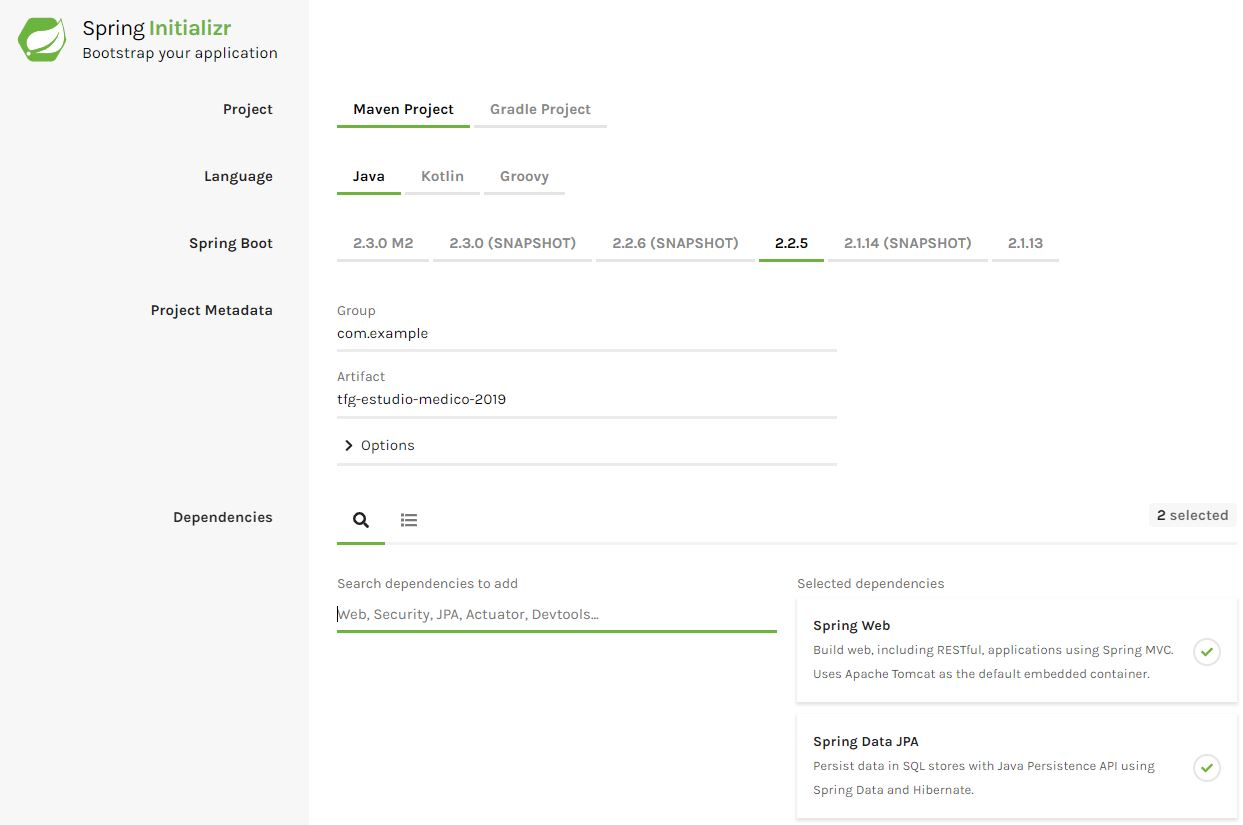
\includegraphics[width=1\textwidth]{images/springstarter}
    \caption{Proyecto inicial Spring Boot}
    \end{figure}
    
     \FloatBarrier

    Una vez generado el proyecto Spring Boot, hubo de importarse el mismo en el entorno de desarrollo Eclipse.
    
    
    \subsection{Arquitectura de la aplicación Java Spring Boot}
    La arquitectura de la aplicación Spring Boot desarrollada se divide principalmente en los apartados de código, documentación y tests.

        \subsubsection{\underline{Código}}
        El proyecto \textit{backend} de la aplicación está escrito en Java 8, y dividido en los siguientes bloques o paquetes, los cuales se describen a continuación.
        
        \begin{itemize}
            \item\textbf{Controladores}  \\
            Son los elementos del código encargados de recibir las diferentes peticiones HTTP y mapear los objetos enviados en las mismas, ya sea en el cuerpo de la petición en caso de ser una petición de tipo POST, o en la propia url si es una petición de tipo GET. Además de esto, son los encargados de realizar la lógica de navegación, llamando a la capa de Negocio y, con el resultado obtenido, generar una respuesta a la parte \textit{frontend} de la aplicación.
            \newline
            
            Para identificar los diferentes controladores de nuestra aplicación, la nomenclatura de los mismos siempre terminará con la palabra \textit{Controller}.
            \newline
            
            En nuestra aplicación disponemos de 3 controladores: El \textit{UserController}, encargado principalmente del proceso de login de la aplicación. El \textit{AdminController}, encargado de obtener todos los recursos que demande el usuario de tipo administrador en nuestra aplicación. Finalmente el \textit{ResearcherController}, encargado de obtener los recursos que demanden los usuarios de tipo investigador en nuestra aplicación.
            \newline
            
            Todos los controladores se han implementado con el patrón de Diseño \textit{Interface}, separando los métodos de su implementación y haciendo al código más legible y mantenible de cara al futuro.
            \newline
            
                \begin{figure}[h]
                    \centering
                     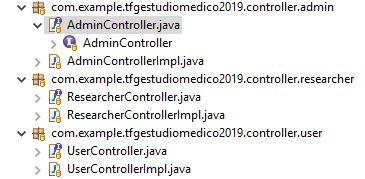
\includegraphics[width=0.8\textwidth]{images/controllers.JPG}
                    \caption{Controladores del proyecto \textit{backend}}
                \end{figure}
                
                \begin{figure}[h]
                \centering
                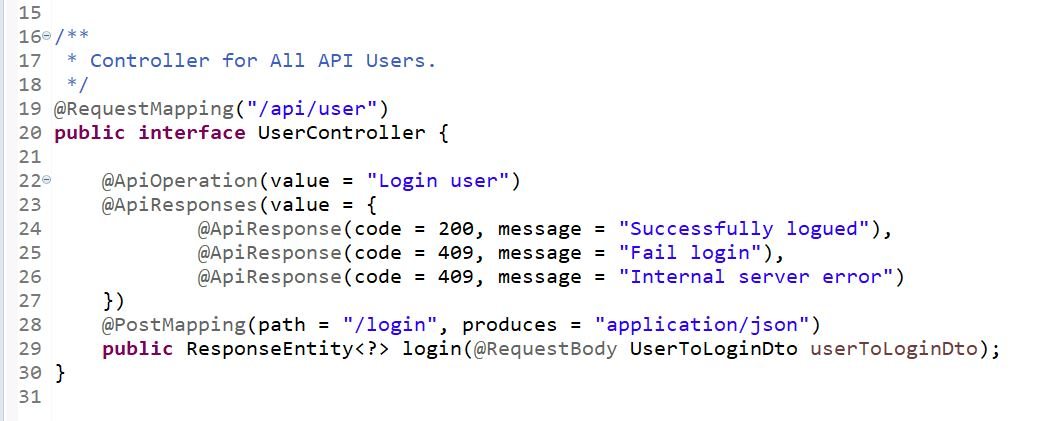
\includegraphics[width=1\textwidth]{images/usercontroller.JPG}
                \caption{Ejemplo Interfaz Controlador UserController}
                \end{figure}
                
                \FloatBarrier
            
             \item\textbf{Servicios de la aplicación}  \\
            Son los elementos del código encargados de centralizar la lógica principal de la aplicación. Los controladores los llaman, estos llaman a los repositorios para obtener los recursos solicitados, y devuelven dichos recursos al controlador.
            \newline
            
            Para identificar los diferentes servicios de de nuestra aplicación, la nomenclatura de los mismos siempre terminará con la palabra \textit{Business}.
            \newline
            
            En nuestra aplicación disponemos de 3 servicios de aplicación: El \textit{UserBusiness}, encargado principalmente de gestionar a los diferentes usuarios de la aplicación. El \textit{ResearcherBusiness}, encargado de gestionar las diferentes funcionalidades que puede realizar un usuario de tipo investigador en nuestra aplicación. Por último el \textit{SubjectBusiness}, encargado de gestionar a los pacientes y a sus respectivas citas y cuestionarios.
            \newline
            
            Al igual que los controladores, todos los servicios de aplicación se han implementado con el patrón de diseño \textit{Interface}
            \newline.
            
             \begin{figure}[h]
                \centering
                
\includegraphics[width=0.8\textwidth]{images/business.JPG}
                \caption{Servicios de Aplicación del proyecto \textit{backend}}
            \end{figure}
            
            \begin{figure}[h]
                \centering
                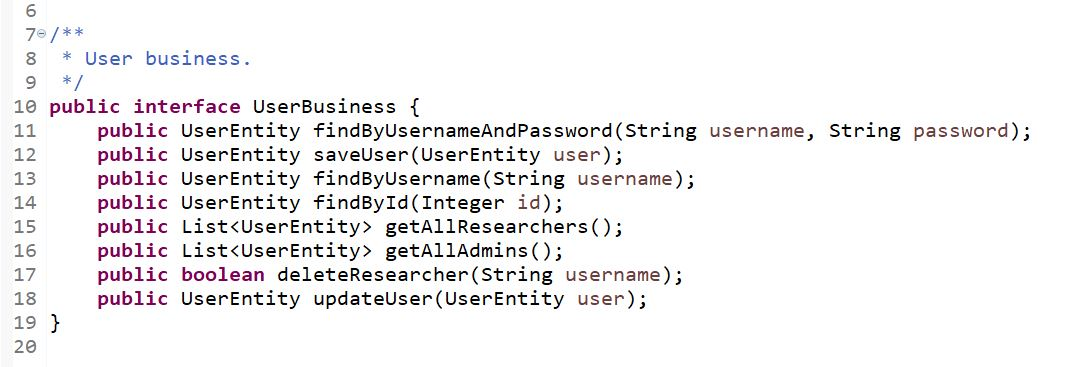
\includegraphics[width=1\textwidth]{images/userbusiness.JPG}
                \caption{Ejemplo Interfaz Servicio de aplicación UserBusiness}
            \end{figure}
            
            \FloatBarrier
            
            \item\textbf{Repositorios}  \\
            Son los elementos encargados de comunicarse con la base de datos correspodiente, ya sea guardando recursos, actualizar, listar, borrar etc... \\
            \newline
            Todos los repositorios extienden de la clase \textit{JpaRepository}, una clase perteneciente a SpringData, la cual implementa el código necesario para realizar una llamada a la base de datos. De esta manera no ha sido necesario implementar dichas clases.
            \newline 
            
            Para identificar los diferentes repositorios de de nuestra aplicación, la nomenclatura de los mismos siempre terminará con la palabra \textit{Repository}.
            \newline
            
            Nuestra aplicación dispone de 4 repositorios: El \textit{InvestigationDetailsRepository}, encargado de gestionar los detalles de los cuestionarios realizados a los pacientes. El \textit{InvestigationRepository}, encargado de gestionar los cuestionarios realizados a los pacientes. El \textit{UserRepository}, encargado de gestionar a los diferentes usuarios administradores e investigadores de la aplicación. Y finalmente, el
            \textit{SubjectRepository}, encargado de gestionar a los pacientes del estudio.
            \newline
            
            \begin{figure}[h]
                \centering
                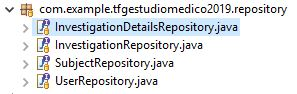
\includegraphics[width=0.8\textwidth]{images/repository.JPG}
                \caption{Repositorios del proyecto \textit{backend}}
            \end{figure}
            
            \begin{figure}[h]
                \centering
                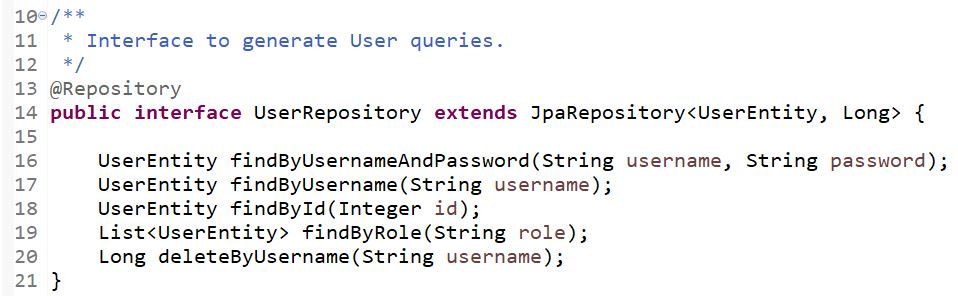
\includegraphics[width=1\textwidth]{images/userrepository.JPG}
                \caption{Interfaz Repositorio UserRepository}
            \end{figure}
            
            \FloatBarrier
            
            \item\textbf{Modelos}  \\
            Son los elementos encargados de almacenar la información de las bases de datos y de las peticiones HTTP, delimitando el dominio de las mismas.
            \newline
            
            Hay 3 tipos de modelos en nuestra aplicación:
            \begin{itemize}
                \item Dominio. \\
                Son los elementos que definen un rango de posibles valores. En nuestra aplicación disponemos del enumerado  \textit{Role} para definir los tipos de usuarios que pueden acceder a la aplicación.
                \newline
                
                 \begin{figure}[h]
                \centering
                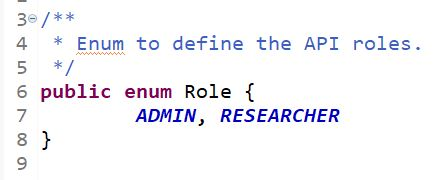
\includegraphics[width=0.9\textwidth]{images/role.JPG}
                \caption{Ejemplo Dominio Enumerado Role}
                \end{figure}
                
                 \FloatBarrier
                
              
                \item Entidades.  \\
                Son los elementos encargados de interactuar con las bases de datos de nuestra aplicación. Estas entidades JPA, también llamadas POJO's(Plain Old Java Objects), se encuentran mapeadas mediante anotaciones y representan las tablas de nuestra base de datos relacional.
                \newline
                
                
            Para identificar las diferentes entidades de nuestra aplicación, la nomenclatura de las mismas siempre terminará con la palabra \textit{Entity}.
            \newline
                
                  \begin{figure}[h]
                        \centering
                        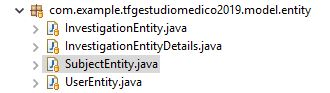
\includegraphics[width=0.8\textwidth]{images/entity.JPG}
                        \caption{Entidades del proyecto \textit{backend}}
                    \end{figure}
            
                    \begin{figure}[h]
                        \centering
                        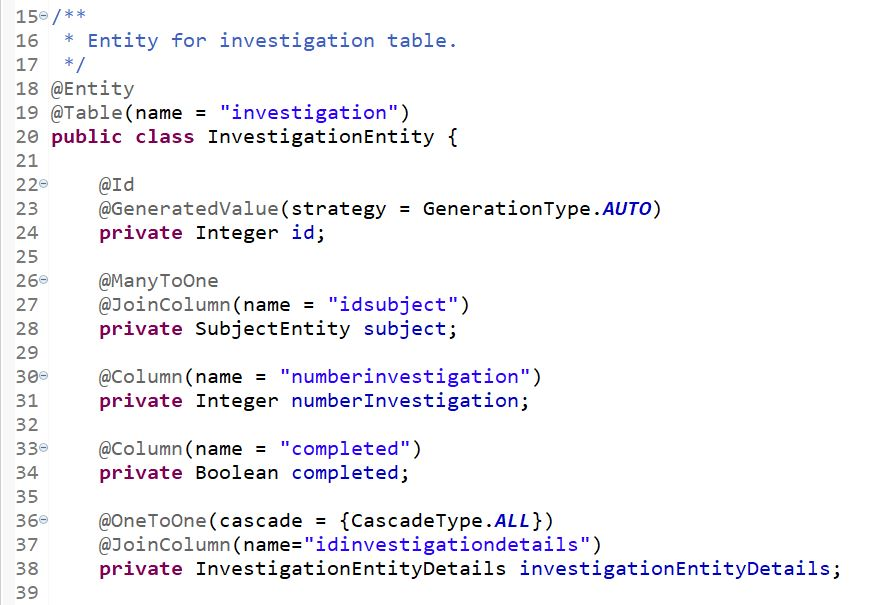
\includegraphics[width=1\textwidth]{images/investigationentity.JPG}
                        \caption{Ejemplo Entidad InvestigationEntity}
                    \end{figure}
            
            \FloatBarrier
                
                
                \item Dtos(Data Transfer Objects). \\
                Son los elementos encargados de mapear los objetos de tipo JSON enviados en las peticiones HTTP para ser tratados en la aplicación. También se encargan de devolver la información necesaria mediante una respuesta HTTP.
                \newline
                
                 Para identificar a los dtos(Data Transfer Objects) de nuestra aplicación, la nomenclatura de los misms siempre terminará con la palabra \textit{Dto}.
                \newline
                
                De esta manera, los controladores de la aplicación tratarán los dtos y los mapearán a entidades para ser tratadas en la capa de Negocio, proporcionando seguridad y robustez a la aplicación, evitando posibles inyecciones de código y protegiendo los campos sensibles que no deban mostrarse en el exterior.
                \newline 
                
                    \begin{figure}[h]
                        \centering
                        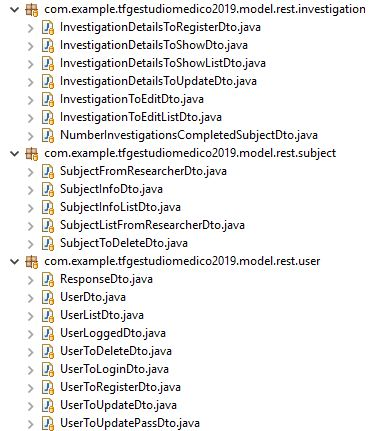
\includegraphics[width=0.8\textwidth]{images/dto.JPG}
                        \caption{Dtos del proyecto \textit{backend}}
                    \end{figure}
            
                    \begin{figure}[h]
                        \centering
                        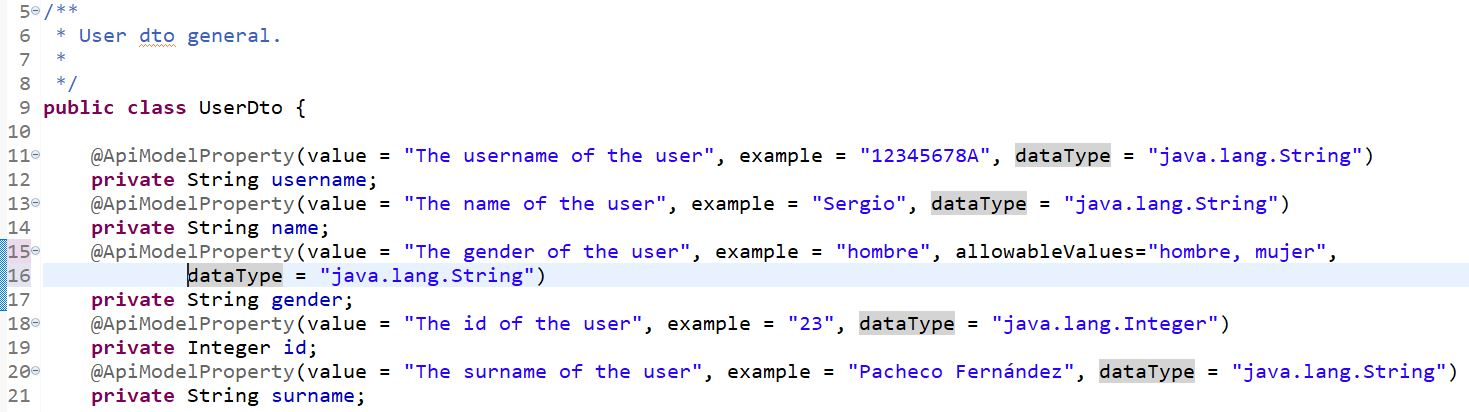
\includegraphics[width=1\textwidth]{images/userdto.JPG}
                        \caption{Ejemplo dto UserDto}
                    \end{figure}
            
            \FloatBarrier
                
                
            \end{itemize}
            
            
        \end{itemize}
        \subsubsection{\underline{Documentación}}
        A la hora de documentar la aplicación \textit{backend}, por una parte, se utilizó \textit{Javadoc} al principio de cada clase Java, y por otro lado, se utilizó \textit{Swagger}. 
        \newline
        
        Para utilizar el \textit{framework} \textit{Swagger} en la aplicación, hubo de añadir las correspondientes dependencias en el archivo \textit{pom.xml}.
        \newline
        
        \begin{figure}[h]
            \centering
            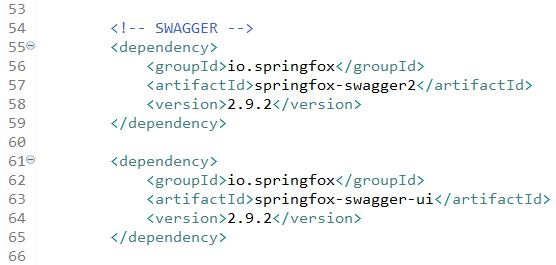
\includegraphics[width=1\textwidth]{images/swagger.JPG}
            \caption{Dependencias Swagger añadidas en pom.xml}
        \end{figure}
        
        \textit{Swagger} nos permitió documentar tanto los puntos de acceso como los dtos de nuestra aplicación a través de anotaciones, las cuales se añadieron en las respectivas clases implicadas.
        
          \begin{figure}[h]
            \centering
            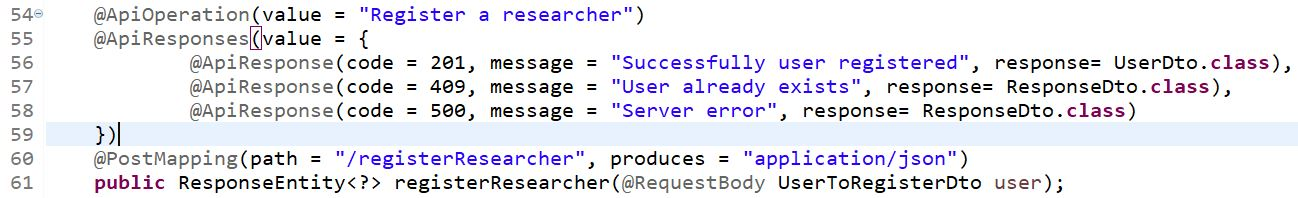
\includegraphics[width=1\textwidth]{images/swaggerexample.JPG}
            \caption{Ejemplo Documentación \textit{Swagger} en el endpoint Registrar Investigador}
        \end{figure}
        
        
         \textit{Swagger} posee una interfaz llamada swagger.ui a la cual se puede acceder una vez arrancado el proyecto \textit{backend} para realizar pruebas y comprobar la documentación generada, como se muestra continuación. Dicha interfaz documenta tanto la información general de la aplicación, como los puntos de acceso y los dtos.
         \newline
         
          \begin{figure}[h]
            \centering
            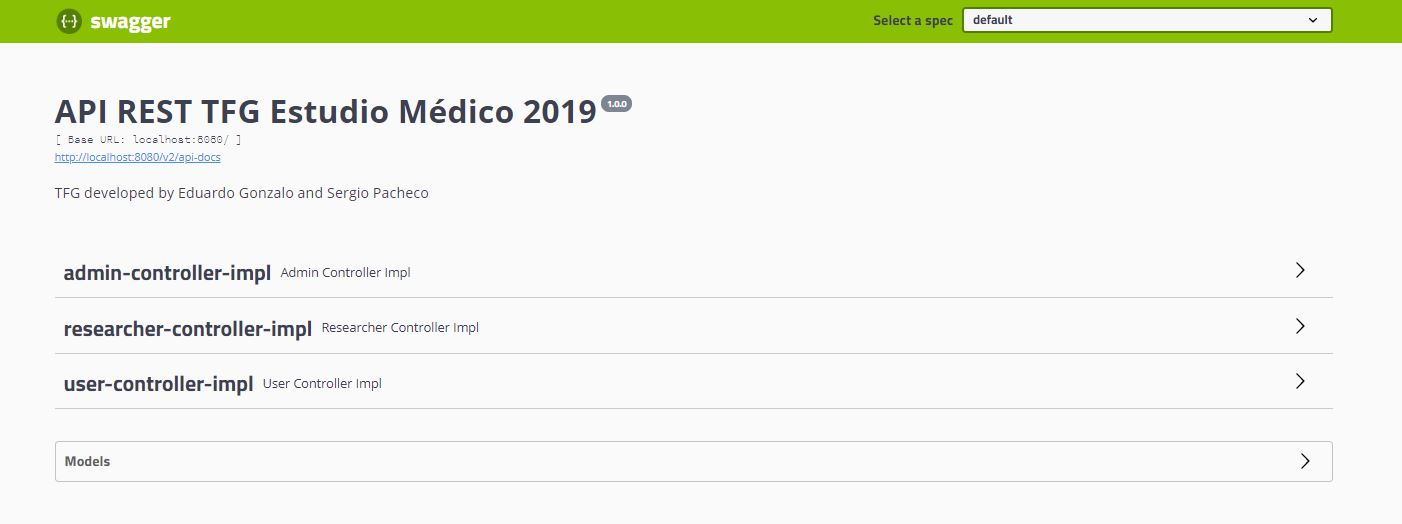
\includegraphics[width=1\textwidth]{images/swaggergeneral.JPG}
            \caption{Interfaz swagger.ui}
        \end{figure}
        
          \begin{figure}[h]
            \centering
            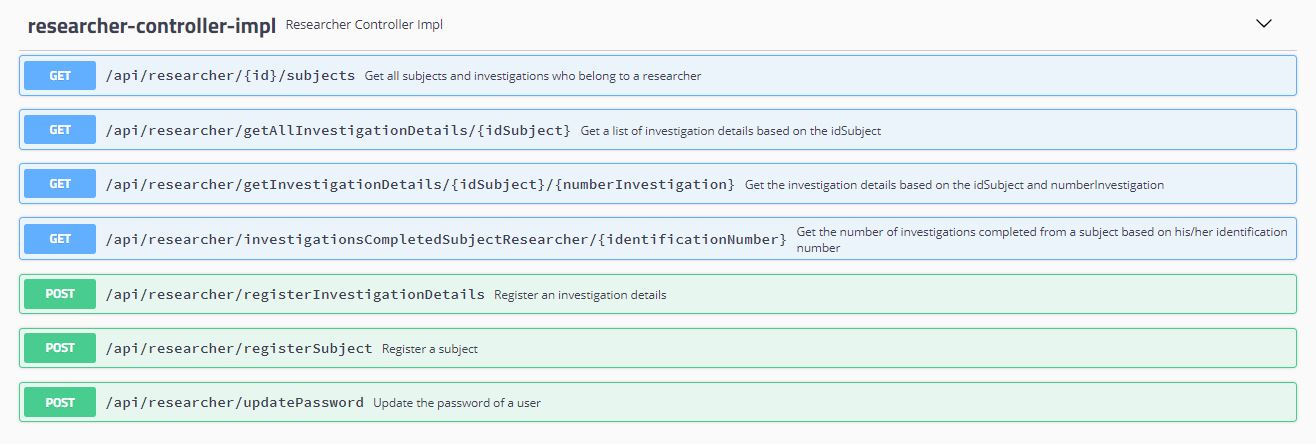
\includegraphics[width=1\textwidth]{images/swaggerendpoint.JPG}
            \caption{Ejemplo Documentación Swagger Researcher Controller}
        \end{figure}
        
        \begin{figure}[h]
            \centering
            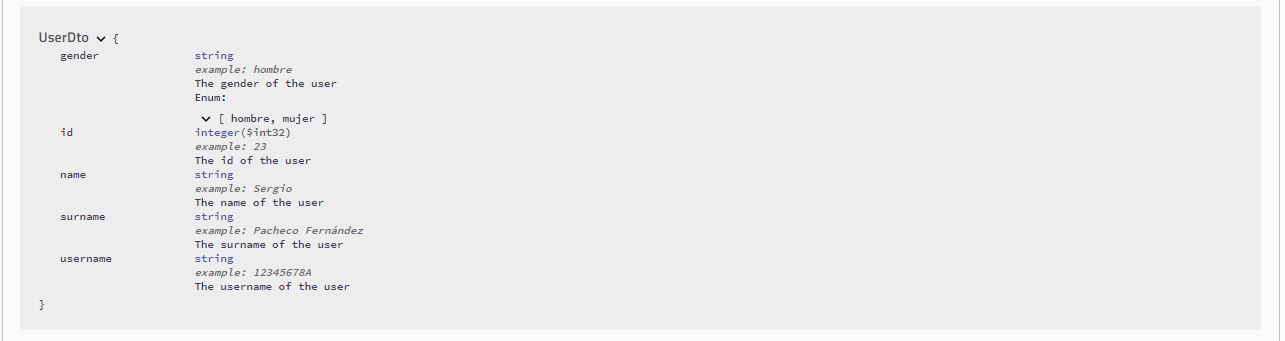
\includegraphics[width=1\textwidth]{images/swaggeruserdto.JPG}
            \caption{Ejemplo Documentación Swagger UserDto}
        \end{figure}
        
        \FloatBarrier
        
        
        \subsubsection{\underline{Tests}}
        A la hora de garantizar la calidad del \textit{software}, se han realizado tests con Mockito y JUnit. Se han testeado todos los métodos de todas las clase que poseen lógica(Controladores y Servicios de Aplicación), probando todos los caminos y excepciones posibles, así como el camino feliz.
        \newline
        
        En la aplicación hay un total de 157 tests realizados, los cuales se ejecutan cada vez que se instala la aplicación, garantizando así el correcto funcionamiento de la misma.
        \newline
        
          \begin{figure}[h]
            \centering
            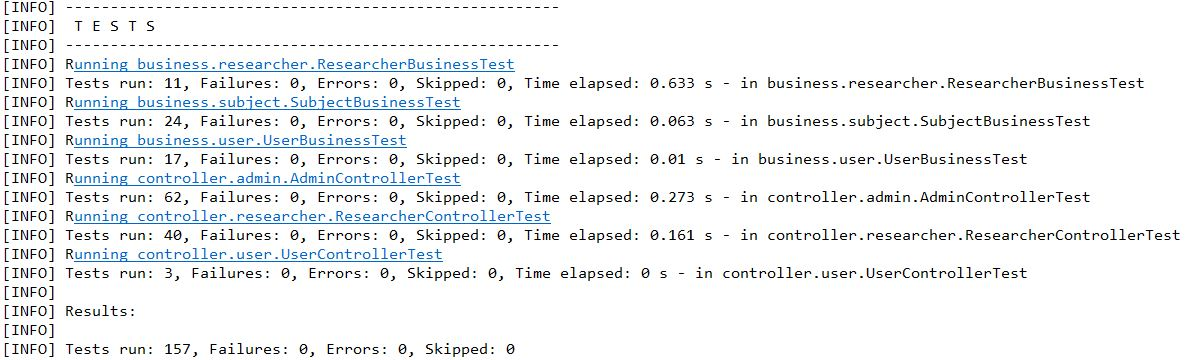
\includegraphics[width=1\textwidth]{images/numtests.JPG}
            \caption{Tests realizados en la aplicación}
        \end{figure}
        
        Para garantizar que se han testeado todos los caminos posibles, se ha conseguido un 100\% de cobertura en todas las clases con tests.
        \newline
        
        
          \begin{figure}[h]
            \centering
            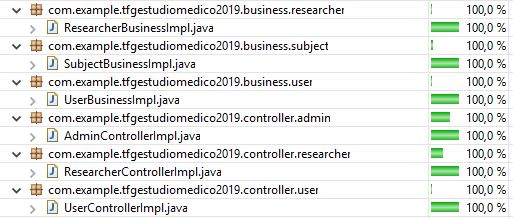
\includegraphics[width=1\textwidth]{images/coberturatests.JPG}
            \caption{Cobertura de las clases testeadas}
        \end{figure}
        \FloatBarrier
        

        
        
    \subsection{Inicialización del proyecto}
        A la hora de inicializar la aplicación \textit{backend}, al tratarse de un proyecto  Maven, lo primero que hay que ejecutar son los siguientes comandos: 
        
        \begin{enumerate}
          \item\texttt{mvn clean}.\\
          Elimina los archivos generados anteriormente y descarga las librerías añadidas como dependencias en el archivo pom.xml
          \item\texttt{mvn install}. \\
          Genera el archivo .jar definido en el pom.xml
        \end{enumerate}
        
        Si queremos ejecutar la aplicación \textit{backend} de manera local, lo único que tenemos que hacer es ejecutar la clase \texttt{Main} de la aplicación en el entorno de desarrollo elegido, en este caso, Eclipse. \\
        \newline
        Si queremos ejecutar la aplicación \textit{backend} de manera remota, solo tenemos que almacenar el archivo .jar generado anteriormente en el servicio de Hosting escogido, en este caso, en Hostinger\cite{hostinger}.
        
        
        
        
    